% Options for packages loaded elsewhere
\PassOptionsToPackage{unicode}{hyperref}
\PassOptionsToPackage{hyphens}{url}
\PassOptionsToPackage{dvipsnames,svgnames,x11names}{xcolor}
%
\documentclass[
  authoryear,
  review]{elsarticle}

\usepackage{amsmath,amssymb}
\usepackage{iftex}
\ifPDFTeX
  \usepackage[T1]{fontenc}
  \usepackage[utf8]{inputenc}
  \usepackage{textcomp} % provide euro and other symbols
\else % if luatex or xetex
  \usepackage{unicode-math}
  \defaultfontfeatures{Scale=MatchLowercase}
  \defaultfontfeatures[\rmfamily]{Ligatures=TeX,Scale=1}
\fi
\usepackage{lmodern}
\ifPDFTeX\else  
    % xetex/luatex font selection
\fi
% Use upquote if available, for straight quotes in verbatim environments
\IfFileExists{upquote.sty}{\usepackage{upquote}}{}
\IfFileExists{microtype.sty}{% use microtype if available
  \usepackage[]{microtype}
  \UseMicrotypeSet[protrusion]{basicmath} % disable protrusion for tt fonts
}{}
\makeatletter
\@ifundefined{KOMAClassName}{% if non-KOMA class
  \IfFileExists{parskip.sty}{%
    \usepackage{parskip}
  }{% else
    \setlength{\parindent}{0pt}
    \setlength{\parskip}{6pt plus 2pt minus 1pt}}
}{% if KOMA class
  \KOMAoptions{parskip=half}}
\makeatother
\usepackage{xcolor}
\setlength{\emergencystretch}{3em} % prevent overfull lines
\setcounter{secnumdepth}{5}
% Make \paragraph and \subparagraph free-standing
\makeatletter
\ifx\paragraph\undefined\else
  \let\oldparagraph\paragraph
  \renewcommand{\paragraph}{
    \@ifstar
      \xxxParagraphStar
      \xxxParagraphNoStar
  }
  \newcommand{\xxxParagraphStar}[1]{\oldparagraph*{#1}\mbox{}}
  \newcommand{\xxxParagraphNoStar}[1]{\oldparagraph{#1}\mbox{}}
\fi
\ifx\subparagraph\undefined\else
  \let\oldsubparagraph\subparagraph
  \renewcommand{\subparagraph}{
    \@ifstar
      \xxxSubParagraphStar
      \xxxSubParagraphNoStar
  }
  \newcommand{\xxxSubParagraphStar}[1]{\oldsubparagraph*{#1}\mbox{}}
  \newcommand{\xxxSubParagraphNoStar}[1]{\oldsubparagraph{#1}\mbox{}}
\fi
\makeatother


\providecommand{\tightlist}{%
  \setlength{\itemsep}{0pt}\setlength{\parskip}{0pt}}\usepackage{longtable,booktabs,array}
\usepackage{calc} % for calculating minipage widths
% Correct order of tables after \paragraph or \subparagraph
\usepackage{etoolbox}
\makeatletter
\patchcmd\longtable{\par}{\if@noskipsec\mbox{}\fi\par}{}{}
\makeatother
% Allow footnotes in longtable head/foot
\IfFileExists{footnotehyper.sty}{\usepackage{footnotehyper}}{\usepackage{footnote}}
\makesavenoteenv{longtable}
\usepackage{graphicx}
\makeatletter
\newsavebox\pandoc@box
\newcommand*\pandocbounded[1]{% scales image to fit in text height/width
  \sbox\pandoc@box{#1}%
  \Gscale@div\@tempa{\textheight}{\dimexpr\ht\pandoc@box+\dp\pandoc@box\relax}%
  \Gscale@div\@tempb{\linewidth}{\wd\pandoc@box}%
  \ifdim\@tempb\p@<\@tempa\p@\let\@tempa\@tempb\fi% select the smaller of both
  \ifdim\@tempa\p@<\p@\scalebox{\@tempa}{\usebox\pandoc@box}%
  \else\usebox{\pandoc@box}%
  \fi%
}
% Set default figure placement to htbp
\def\fps@figure{htbp}
\makeatother

\usepackage{booktabs}
\usepackage{caption}
\usepackage{longtable}
\usepackage{colortbl}
\usepackage{array}
\usepackage{anyfontsize}
\usepackage{multirow}
\makeatletter
\@ifpackageloaded{caption}{}{\usepackage{caption}}
\AtBeginDocument{%
\ifdefined\contentsname
  \renewcommand*\contentsname{Table of contents}
\else
  \newcommand\contentsname{Table of contents}
\fi
\ifdefined\listfigurename
  \renewcommand*\listfigurename{List of Figures}
\else
  \newcommand\listfigurename{List of Figures}
\fi
\ifdefined\listtablename
  \renewcommand*\listtablename{List of Tables}
\else
  \newcommand\listtablename{List of Tables}
\fi
\ifdefined\figurename
  \renewcommand*\figurename{Figure}
\else
  \newcommand\figurename{Figure}
\fi
\ifdefined\tablename
  \renewcommand*\tablename{Table}
\else
  \newcommand\tablename{Table}
\fi
}
\@ifpackageloaded{float}{}{\usepackage{float}}
\floatstyle{ruled}
\@ifundefined{c@chapter}{\newfloat{codelisting}{h}{lop}}{\newfloat{codelisting}{h}{lop}[chapter]}
\floatname{codelisting}{Listing}
\newcommand*\listoflistings{\listof{codelisting}{List of Listings}}
\makeatother
\makeatletter
\makeatother
\makeatletter
\@ifpackageloaded{caption}{}{\usepackage{caption}}
\@ifpackageloaded{subcaption}{}{\usepackage{subcaption}}
\makeatother
\journal{Open Quaternary}

\usepackage[]{natbib}
\bibliographystyle{elsarticle-harv}
\usepackage{bookmark}

\IfFileExists{xurl.sty}{\usepackage{xurl}}{} % add URL line breaks if available
\urlstyle{same} % disable monospaced font for URLs
\hypersetup{
  pdftitle={Biogeography of crop progenitors and wild plant resources over the Pleistocene/Holocene boundary in West Asia, 14.7--8.3 ka},
  pdfauthor={Joe Roe; Amaia Arranz-Otaegui},
  colorlinks=true,
  linkcolor={blue},
  filecolor={Maroon},
  citecolor={Blue},
  urlcolor={Blue},
  pdfcreator={LaTeX via pandoc}}


\setlength{\parindent}{6pt}
\begin{document}

\begin{frontmatter}
\title{Biogeography of crop progenitors and wild plant resources over
the Pleistocene/Holocene boundary in West Asia, 14.7--8.3 ka}
\author[1,2]{Joe Roe%
\corref{cor1}%
}
 \ead{joeroe@hey.com} 
\author[3]{Amaia Arranz-Otaegui%
%
}


\affiliation[1]{organization={University of
Bern},country={Switzerland},countrysep={,},postcodesep={}}
\affiliation[2]{organization={University of
Copenhagen},country={Denmark},countrysep={,},postcodesep={}}
\affiliation[3]{organization={University of the Basque
Country},country={Spain},countrysep={,},postcodesep={}}

\cortext[cor1]{Corresponding author}


        
\begin{abstract}
This paper presents the first comprehensive reconstructions of the
palaeodistributions of 56 plant species found regularly in association
with early agricultural archaeological sites in West Asia, including the
progenitors of the first crops. We used machine learning to train an
ecological niche model of each species based on its present-day
distribution in relation to climate and environmental variables.
Predictions of the potential ranges of these species at key stages of
the Pleistocene--Holocene transition could then be derived from these
models using hindcast data from palaeoclimate simulations. Species
ranges are predicted to have been on average {[}X\%{]}
{[}larger\textbar smaller{]} in the Early Holocene compared to present
conditions, but did {[}not{]} change as drastically between the Last
Glacial Maximum and the Early Holocene. However, the modelled ranges do
not predict the observed occurrence of these species on archaeological
sites with any degree of accuracy. The regional ubiquity of species in
the archaeological record is {[}not{]} correlated with the predicted
size of its range and the diversity of archaeobotanical assemblages is
{[}not{]} correlated with the predicted diversity of its environs. This
indicates that trends in taxonomic composition of the archaeobotanical
record is {[}not{]} likely to have been influenced by environmental
change and species turnover, in addition to human economic choices.
\end{abstract}





\end{frontmatter}
    

\begin{itemize}
\tightlist
\item[$\boxtimes$]
  Finish modelling
\item[$\square$]
  First draft:

  \begin{itemize}
  \tightlist
  \item[$\square$]
    Introduction
  \item[$\square$]
    Background

    \begin{itemize}
    \tightlist
    \item[$\square$]
      Biogeography
    \item[$\boxtimes$]
      ENM
    \end{itemize}
  \item[$\boxtimes$]
    Methods \& Materials
  \item[$\square$]
    Results

    \begin{itemize}
    \tightlist
    \item[$\square$]
      Model assessment
    \end{itemize}
  \item[$\square$]
    Discussion

    \begin{itemize}
    \tightlist
    \item[$\square$]
      General trends
    \item[$\square$]
      Case studies
    \end{itemize}
  \item[$\square$]
    Conclusion
  \end{itemize}
\item[$\square$]
  Figures

  \begin{itemize}
  \tightlist
  \item[$\square$]
    tbl-occ-count (needs pdf cleanup)
  \item[$\square$]
    tbl-predictors
  \item[$\square$]
    tbl-climate-periods
  \end{itemize}
\item[$\square$]
  Clean up package code
\item[$\square$]
  Appendix with all hindcast predictions
\item[$\square$]
  References \& copyediting
\item[$\square$]
  Final proofread
\end{itemize}

\section{Introduction}\label{introduction}

\begin{itemize}
\tightlist
\item
  The first farming societies had an ecological context
\item
  Subsistence is understood (largely) through archaeobotany and
  zooarchaeology; ecological context from environmental archaeology,
  palynology, palaeoclimate records, etc.

  \begin{itemize}
  \tightlist
  \item
    But these have a variety of biases (human selection, taphonomy,
    etc.)
  \item
    And at the end of the day only represent specific places --
    interpolation to the entire region is not straightforward
  \item
    Overlap makes it difficult to see where human choices depart from
    the environmental background \citep[cf.][]{MartinEtAl2016}
  \item
    Or to fully contextualise subsistence strategies and shifts in
    strategies in response to environmental shifts
    \citep[e.g.][]{YaworskyEtAl2023}.
  \end{itemize}
\item
  Here we present an alternative approach using ENM

  \begin{itemize}
  \tightlist
  \item
    Whole region, at multiple climate snapshots
  \item
    Independent of archaeobot. and pal. clim. data, so can verify and
    compare
  \end{itemize}
\end{itemize}

\section{Background}\label{background}

\begin{itemize}
\tightlist
\item
  The transition to agriculture in West Asia was\ldots{}
\end{itemize}

\subsection{Biogeography and agricultural
origins}\label{biogeography-and-agricultural-origins}

\begin{itemize}
\tightlist
\item
  Has always been important in study of agricultural origins

  \begin{itemize}
  \tightlist
  \item
    Historically: Vavilov, Pumpelly \& Childe
  \item
    Genetic studies tell us origin points, but not ranges
  \end{itemize}
\item
  Important to e.g.

  \begin{itemize}
  \tightlist
  \item
    Distinguish environmental from potentially anthropogenic change
    \citep{MartinEtAl2017, MartinEtAl2025}
  \item
    Reconstruct sequences of domestication \citep{YeomansEtAl2017}
  \end{itemize}
\item
  Epipal./Neo. plant-based economies were diverse

  \begin{itemize}
  \tightlist
  \item
    More than the ``founder crops'';
  \item
    More than food
  \item
    (In archaebot., not all intentionally collected)
  \item
    Regionally and temporally diverse
  \item
    \ldots so we model lots of species!
  \end{itemize}
\item
  Regional ecological reconstructions generally rely on the `expert
  interpolation' (or what do they call it with isoscapes?) method

  \begin{itemize}
  \tightlist
  \item
    See CSEAS (AEA-prep) presentation
  \item
    Figure: comparisons
  \end{itemize}
\end{itemize}

\subsection{Ecological niche modelling in
archaeology}\label{ecological-niche-modelling-in-archaeology}

Ecological niche modelling (ENM) or species distribution modelling (SDM)
is widely used by ecologists to predict the geographic range of a
species based on a set of environmental predictors. Essentially, it
involves combining records of where an organism has been observed with
environmental data (climate, topography, etc.) for those locations to
model the range of environmental values at which that species -- its
environmental niche. This model can then be used to predict the range of
the organism in question either in the same or a different environment.
\citet{CITE} suggests reserving the term `species distribution
modelling' for when the method is used to recover the verifiable range
of a species in a real and existing environment, and using `ecological
niche modelling' as the broader term covering hypothetical or predictive
applications -- a convention we follow here when referring to predictive
or `hindcast' models of past ranges. Within this overarching framework,
ecological niche modelling encompasses a wide range of applications and
a variety of potential environmental predictors, modelling approaches,
and methodologies, which we will not attempt to review here.

Ecological niche modelling has long been of interest to archaeologists
as both a means of exploring the biological niche of humans and for
reconstructing the past environments they inhabited
\citep{DavidPollyEronen2011, FranklinEtAl2015}. In the first sense, it
has been used most extensively to model the range of humans and other
hominin species
\citep[e.g.][]{BenitoEtAl2017, YousefiEtAl2020, BanksEtAl2021, YaworskyEtAl2024a, YaworskyEtAl2024b, GuranEtAl2024},
especially in the Palaeolithic. This overlaps with what archaeologists
usually call generically `predictive modelling'
\citep{VerhagenWhitley2020}---more precisely `site distribution
modelling'---which is essentially the same approach as (and often
borrows methodologies from) ecological niche modelling but applied to
the occurrence of archaeological sites. Here what is modelled is not
strictly a biological niche alone, but also aspects of human geography,
taphonomy, and archaeological visibility. These applications can be
distinguihed from `palaeoecological niche modelling', where the object
of model remains, as in ecology, a non-human biological niche.

\citet{FranklinEtAl2015} review palaeoecological niche modelling and
advocate for its greater adoption in environmental archaeology. In an
early application to West Asia, \citet{ConollyEtAl2012} used the
occurrence of wild and domestic \emph{Bos} remains at prehistoric
archaeological sites to map the evolving niche of cattle over the
Pleistocene--Holocene transition. It has been used to model the
availability of fauna exploited by humans at wider scales
\citep[e.g.][]{deAndresHerreroEtAl2018, YaworksyEtAl2023} and, in a West
Asian context, of foraged plant resources in the landscape around the
Neolithic site of XX \citep{CollinsEtAl2018}. Modelling the spread of
crops has been another significant archaeological application
\citep{CremaEtAl}.

In the majority of studies to date (palaeo)ecological niche modelling
has been applied to archaeological data in an `inductive' fashion,
i.e.~faunal and botanical remains from ancient sites are used as the
occurrence dataset for training a model using either past or present
environmental data. However, both the zooarchaeological and
archaeobotanical records are sparse and subject to a complex array of
depositional, taphonomic and recovery biases factors that , many of
which are not fully understood and/or cannot be corrected for. This
means that while the archaeological attestation of the presence of a
species might generally be relied upon, it is highly unlikely that its
absence is representative of true past distributions.

The alternative approach is to train the model using contemporary
occurrence and environmental data and then use palaeoenvironmental data
to `hindcast' its predictions backwards in time. Like
\citet{FranklinEtAl2015}, we view the hindcasting approach as more
promising, because training datasets for both occurrences and
environment are far more readily available, complete and reliable for
the present than the past. There is some scepticism in the ecological
niche modelling literature about the ability of such models to make
accurate predictions in unknown environments (like the past)
\citep{CITES}, but here the hindcasting approach also presents an
opportunity: it reserves archaeological occurrence data as an
independent dataset that can be used to assess the retrodictive
performance of the model. This possibily was suggested by
\citet{FranklinEtAl2015} but to our knowledge our study represents the
first attempt to actually do so.

The major practical limitation of the hindcasting approach is that it
relies on spatially explicit, high resolution palaeoenvironmental
surfaces with continuous coverage of the region and periods of interest.
Until recently, this has not been widely available for most
applications, which is perhaps why only a minority of studies use it
\citep[cf.][]{YaworskyEtAl2023}. In this study, we are able to take
advantage of the increasing availability of high resolution, global
palaeoclimate data derived from simulation experiments with general
circulation models of climate
\citep{BrownEtAl2018, BrownEtAl2020, KargerEtAl2023}.

\section{Methods and materials}\label{methods-and-materials}

\begin{figure}

\centering{

\pandocbounded{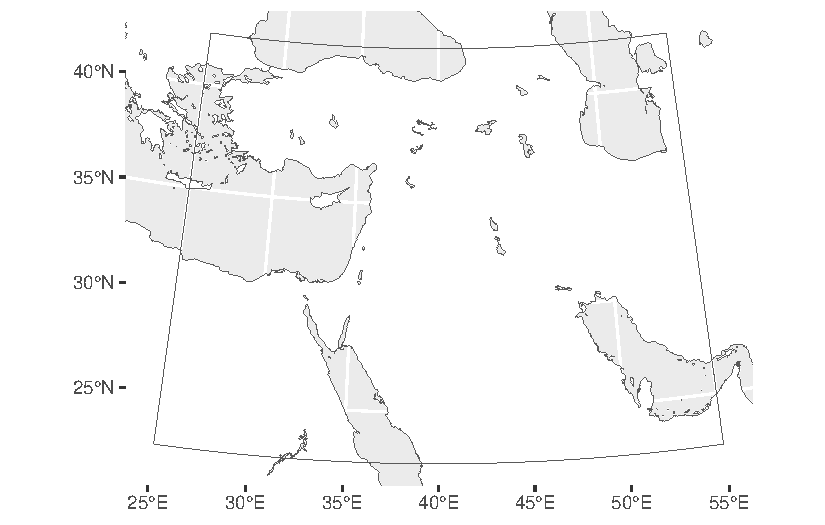
\includegraphics[keepaspectratio]{paper_files/figure-pdf/fig-region-1.pdf}}

}

\caption{\label{fig-region}Study region (red) and archaeological sites
used to generate modelled flora. Solid circles indicate Neolithic
sites.}

\end{figure}%

We began by considering 62 distinct taxa (Table~\ref{tbl-occ-count}) -
all the identifiable species known to be present at more than three
Neolithic (c.~11.7--6.5 ka) sites in West Asia, according to our
previous study of the regional archaeobotanical data
\citep{ArranzOtaeguiRoe2023}. Taxonomic names were resolved to the
canonical form specified in the GBIF Backbone Taxonomy
\citep{GBIFSecretariat2023}. So for example occurrences for
\emph{Bolboschoenus maritimus} also include those recorded under the
older nomenclature \emph{Scirpus maritimus} (see
Table~\ref{tbl-occ-count}). Domestic species meeting our inclusion
criteria were substituted with their wild progenitor(s), where known.

\subsection{Occurrence data}\label{occurrence-data}

\begin{verbatim}
Warning: HTML tags found, and they will be removed.
* Set `options(gt.html_tag_check = FALSE)` to disable this check.
HTML tags found, and they will be removed.
* Set `options(gt.html_tag_check = FALSE)` to disable this check.
HTML tags found, and they will be removed.
* Set `options(gt.html_tag_check = FALSE)` to disable this check.
HTML tags found, and they will be removed.
* Set `options(gt.html_tag_check = FALSE)` to disable this check.
HTML tags found, and they will be removed.
* Set `options(gt.html_tag_check = FALSE)` to disable this check.
HTML tags found, and they will be removed.
* Set `options(gt.html_tag_check = FALSE)` to disable this check.
HTML tags found, and they will be removed.
* Set `options(gt.html_tag_check = FALSE)` to disable this check.
HTML tags found, and they will be removed.
* Set `options(gt.html_tag_check = FALSE)` to disable this check.
HTML tags found, and they will be removed.
* Set `options(gt.html_tag_check = FALSE)` to disable this check.
HTML tags found, and they will be removed.
* Set `options(gt.html_tag_check = FALSE)` to disable this check.
HTML tags found, and they will be removed.
* Set `options(gt.html_tag_check = FALSE)` to disable this check.
HTML tags found, and they will be removed.
* Set `options(gt.html_tag_check = FALSE)` to disable this check.
\end{verbatim}

\begin{table}

\caption{\label{tbl-occ-count}Recorded occurrence of flora considered in
this study in Neolithic and contemporary West Asia}

\centering{

\fontsize{12.0pt}{14.4pt}\selectfont
\begin{tabular*}{\linewidth}{@{\extracolsep{\fill}}lrr}
\toprule
 & \multicolumn{2}{c}{Occurrences} \\ 
\cmidrule(lr){2-3}
Taxon & Neolithic & Present \\ 
\midrule\addlinespace[2.5pt]
\emph{Triticum turgidum dicoccum}

incl. \emph{Triticum aestivum}, \emph{Triticum dicoccoides}, \emph{Triticum dicoccum} & 64 (44\%) & 200 \\ 
\emph{Hordeum spontaneum}

incl. \emph{Hordeum vulgare} & 62 (43\%) & 6912 \\ 
\emph{Triticum monococcum aegilopoides}

incl. \emph{Triticum boeoticum}, \emph{Triticum monococcum} & 44 (30\%) & 3213 \\ 
\emph{Bolboschoenus maritimus}

incl. \emph{Scirpus maritimus} & 33 (23\%) & 364 \\ 
\emph{Vicia ervilia} & 33 (23\%) & 858 \\ 
\emph{Buglossoides tenuiflora} & 31 (21\%) & 159 \\ 
\emph{Arnebia decumbens} & 25 (17\%) & 240 \\ 
\emph{Buglossoides arvensis} & 25 (17\%) & 251 \\ 
\emph{Medicago radiata} & 21 (14\%) & 883 \\ 
\emph{Androsace maxima} & 20 (14\%) & 130 \\ 
\emph{Vicia orientalis}

incl. \emph{Lens culinaris} & 17 (12\%) & 441 \\ 
\emph{Medicago astroites}

incl. \emph{Trigonella astroites} & 16 (11\%) & 130 \\ 
\emph{Arnebia linearifolia} & 14 (10\%) & 158 \\ 
\emph{Linum bienne}

incl. \emph{Linum usitatissimum} & 11 (8\%) & 274 \\ 
\emph{Gypsophila vaccaria}

incl. \emph{Vaccaria pyramidata} & 11 (8\%) & 326 \\ 
\emph{Carex divisa} & 10 (7\%) & 330 \\ 
\emph{Ficus carica} & 10 (7\%) & 4265 \\ 
\emph{Lathyrus oleraceus}

incl. \emph{Pisum elatius}, \emph{Pisum sativum} & 8 (6\%) & 2269 \\ 
\emph{Vicia faba} & 8 (6\%) & 2578 \\ 
\emph{Aizoanthemopsis hispanica}

incl. \emph{Aizoon hispanicum} & 7 (5\%) & 303 \\ 
\emph{Bolboschoenus glaucus} & 7 (5\%) & 27\textsuperscript{\textit{*}} \\ 
\emph{Pistacia atlantica} & 7 (5\%) & 928 \\ 
\emph{Polygonum arenarium arenarium}

incl. \emph{Polygonum venantianum} & 7 (5\%) & 5\textsuperscript{\textit{*}} \\ 
\emph{Prosopis farcta} & 7 (5\%) & 1205 \\ 
\emph{Rumex pulcher} & 7 (5\%) & 794 \\ 
\emph{Ammi majus} & 6 (4\%) & 461 \\ 
\emph{Cicer reticulatum}

incl. \emph{Cicer arietinum} & 6 (4\%) & 193 \\ 
\emph{Hordeum bulbosum} & 6 (4\%) & 2036 \\ 
\emph{Polygonum corrigioloides} & 6 (4\%) & 4\textsuperscript{\textit{*}} \\ 
\emph{Salsola kali} & 6 (4\%) & 369 \\ 
\emph{Taeniatherum caput-medusae} & 6 (4\%) & 235 \\ 
\emph{Capparis spinosa} & 5 (3\%) & 4031 \\ 
\emph{Chenopodium album} & 5 (3\%) & 357 \\ 
\emph{Lolium temulentum} & 5 (3\%) & 148 \\ 
\emph{Poa bulbosa} & 5 (3\%) & 1401 \\ 
\emph{Aegilops crassa} & 4 (3\%) & 170 \\ 
\emph{Atriplex prostrata} & 4 (3\%) & 112 \\ 
\emph{Brachypodium distachyon} & 4 (3\%) & 1581 \\ 
\emph{Fumaria densiflora} & 4 (3\%) & 194 \\ 
\emph{Gypsophila pilosa} & 4 (3\%) & 79 \\ 
\emph{Hordeum murinum} & 4 (3\%) & 1342 \\ 
\emph{Lathyrus aphaca} & 4 (3\%) & 2085 \\ 
\emph{Lathyrus sativus} & 4 (3\%) & 297 \\ 
\emph{Secale cereale} & 4 (3\%) & 1153 \\ 
\emph{Triticum durum} & 4 (3\%) & 219 \\ 
\emph{Vitis sylvestris} & 4 (3\%) & 3\textsuperscript{\textit{*}} \\ 
\emph{Adonis flammea} & 3 (2\%) & 79 \\ 
\emph{Avena sterilis} & 3 (2\%) & 50001\textsuperscript{\textit{*}} \\ 
\emph{Bassia arabica} & 3 (2\%) & 230 \\ 
\emph{Bromus sterilis} & 3 (2\%) & 385 \\ 
\emph{Cephalaria syriaca} & 3 (2\%) & 144 \\ 
\emph{Glaucium aleppicum} & 3 (2\%) & 22\textsuperscript{\textit{*}} \\ 
\emph{Helianthemum ledifolium} & 3 (2\%) & 668 \\ 
\emph{Lolium rigidum} & 3 (2\%) & 1464 \\ 
\emph{Phalaris paradoxa} & 3 (2\%) & 370 \\ 
\emph{Quercus ithaburensis} & 3 (2\%) & 1431 \\ 
\emph{Triticum aestivum compactum} & 3 (2\%) & 209 \\ 
\emph{Verbena officinalis} & 3 (2\%) & 1046 \\ 
\emph{Vicia narbonensis} & 3 (2\%) & 1529 \\ 
\emph{Triticum urartu} & — & 2033 \\ 
\emph{Aegilops speltoides} & — & 1429 \\ 
\emph{Aegilops tauschii} & — & 1395 \\ 
\bottomrule
\end{tabular*}
\begin{minipage}{\linewidth}
\textsuperscript{\textit{*}}Excluded from modelling due to sample size\\
\end{minipage}

}

\end{table}%

Georeferenced occurrence data was obtained from the Global Biodiversity
Information Facility (GBIF) using via its application programming
interface and the R package `rgbif'
\citep{ChamberlainBoettiger2017, rgbif}. GBIF occurrences marked has
having imprecise or duplicate coordinates were excluded from the
training dataset, as were fossil records. Although niche models have
reasonable predictive power even with small training samples
\citep{StockwellPeterson2002, HernandezEtAl2006, WiszEtAl2008}, we
excluded 57 taxa with less than 50 occurrences in West Asia, following
recommendations for niche models generally and Random Forest-based
models specifically \citep{StockwellPeterson2002, LuanEtAl2020}. We also
excluded one taxon (\emph{Avena sterilis}) with over 50,000 occurrences,
as this would have been computationally prohibitive and we were
uncertain what account for such a disproportionately high number of
records.

Occurrence data only tells us where a species is present; there is
rarely definitive information on where the species is \emph{not} found.
We therefore need to generate random background points or
``pseudo-absences'' to feed to the model. There are several ways to do
this. We follow the advice of \citet{BarbetMassinEtAl2012} for
regression-based species distribution models and use a large (:10000)
random sample of points, weighted equally against the presences in the
regression. \citet{ValaviEtAl2022} also recommend using a very large
background sample for random forest models.

\subsection{Predictor data}\label{predictor-data}

We modelled the occurrence of species as a function of X spatial
predictor variables (\textbf{?@tbl-predictors}). These included:

\begin{itemize}
\tightlist
\item
  Sixteen `bioclimatic' variables derived from monthly temperature and
  precipitation values, following standard practice for species
  distribution models \citep{HijmansEtAl2005}. Contemporary bioclimatic
  predictor data for West Asia was extracted from the global CHELSA
  dataset \citep{KargerEtAl2017}, which predicts temperature and
  precipitation from downscaled general circulation model output at 1 km
  resolution.
\end{itemize}

\begin{itemize}
\tightlist
\item
  Terrain aspect and slope, which at high resolution perform well as
  proxies for solar radiation when modelling plant occurrence
  \citep{AustinVanNiel2011, LeempoelEtAl2015}; and the topographic
  wetness index (TWI), which serves as a proxy for soil moisture and is
  particularly important in modelling arid environments
  \citep{KopeckyCizkova2010, CamposEtAl2016, DiVirgilioEtAl2018}. All
  three were derived from the SRTM15+ digital elevation model using
  algorithms from WhiteboxTools \citep{Lindsay2016}.
\end{itemize}

\begin{itemize}
\tightlist
\item
  Edaphic data from SoilGrids \citep{HenglEtAl2014, HenglEtAl2017},
  which improves model performance for plants
  \citep{DubuisEtAl2013, ModEtAl2016, VelazcoEtAl2017}. Based on a
  recent assessment of the reliability of SoilGrids data for species
  distribution modelling \citep{MillerEtAl2024}, we used a subset of
  four variables relating to soil texture (clay, silt, sand) and pH at
  the surface (0-5 cm depth).
\end{itemize}

Predictor data was transformed to common equal-area projection and
resolution of 5 km.

\begin{table}

\caption{\label{tbl-climate-periods}}

\centering{

\fontsize{12.0pt}{14.4pt}\selectfont
\begin{tabular*}{\linewidth}{@{\extracolsep{\fill}}lr}
\toprule
Period & Age, ka \\ 
\midrule\addlinespace[2.5pt]
Bølling-Allerød (BA) & 14.7–12.9 \\ 
Younger Dryas (YDS) & 12.9–11.7 \\ 
Early Holocene (EH) & 11.7–8.3 \\ 
Current (CUR) & — \\ 
\bottomrule
\end{tabular*}

Palaeoclimatic periods used for hindcasting, after \citet{BrownEtAl2018}

}

\end{table}%

For hindcasting, we used reconstructed bioclimatic data for 3 key
periods (Table~\ref{tbl-climate-periods}) generated from downscaled
paleoclimate simulations from the HadCM3 general circulation model
\citep{BrownEtAl2018}. Terrain and soil predictors were held constant,
since reconstructions of these variables in the past are not available
at sufficient scale. It is not likely that either macroscale topography
or soil characteristics have altered significantly over the period of
time considered here, so we assume that this does not degrade model
performance, and may in fact benefit it by providing `anchoring'
predictors that are independent of climate change.

\subsection{Random Forest}\label{random-forest}

Ecological niche modelling is a classification problem that can be
approached with a wide range of statistical methods. A substantial
literature exists on the relatively performance of these approaches and
their respective parameterisations \citep[reviewed
in][]{ValaviEtAl2022}. Random Forest, a widely-used machine learning
algorithm, is amongst the best performing approaches for presence-only
species distribution models, providing it is appropriately parameterised
to account for the class imbalance between presence and background
samples \citep{ValaviEtAl2021, ValaviEtAl2022}. For our application, it
also has the advantage of requiring little to no manual parameter tuning
to achieve good predictive results, which makes it easier to model a
larger numbers of taxa.

For each taxon we trained a classification model to predict occurrence
(presence or absence/background) based on our X predictor variables
(\textbf{?@tbl-predictors}). We used the Random Forest algorithm
implemented in the R package `ranger' \citep{WrightZiegler2017} and the
`tidymodels' \citep{tidymodels} framework for data preprocessing and
model selection. To avoid overfitting, we follow \citet{ValaviEtAl2021}
in their recommended hyperparameters and use of down-sampling to balance
presence and background samples. Models for each taxon were fit
independently, with redundant zero-variance predictors excluded, and
assessed based on balanced training (¾) and test (¼) partitions.

\section{Results}\label{results}

We trained Random Forest models for 56 taxa using contemporary
occurrence data from GBIF, a random sample of background points, and the
predictor variables described in \textbf{?@tbl-predictors}. Substituting
the ``current'' climate predictors for those derived from palaeoclimatic
simulations \citep{BrownEtAl2018}, we could then generate hindcast
predictions for reconstructed past environments in 4 key climate periods
-- a total of 224 modelled palaeodistributions. Predicted distributions
for individual taxa are presented in the appendix and accompanying
material.

\subsection{Model assessment}\label{model-assessment}

\begin{verbatim}
Warning: Removed 51 rows containing missing values or values outside the scale range
(`geom_text_repel()`).
\end{verbatim}

\begin{figure}

\centering{

\pandocbounded{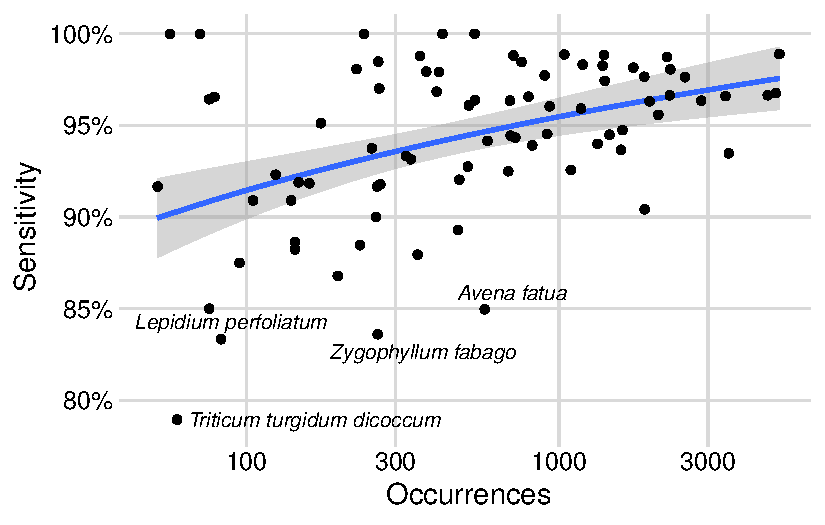
\includegraphics[keepaspectratio]{paper_files/figure-pdf/fig-model-sensitivity-vs-n_occ-1.pdf}}

}

\caption{\label{fig-model-sensitivity-vs-n_occ}Number of taxon
occurrences and model sensitivity on test dataset}

\end{figure}%

We assessed the predictive performance of the fitted niche models in the
contemporary environment based on the reserved test partition. Model
accuracy (proportion of correctly classified presence and background
samples) ranged between 72\% and 98\%, with an average of 91\%.
Sensitivity (proportion of correctly classified presence samples) ranged
between 80\% and 100\%, with an average of 93\%. The area under the
models' receiver operating characteristic curves (ROC-AUC) was in the
range of 0.973±0.058 Model sensitivity is loosely correlated with the
number of occurrences available for training
(Figure~\ref{fig-model-sensitivity-vs-n_occ}), with the worst-performing
models all having less than 300 recorded occurrences: \emph{Buglossoides
tenuiflora}, \emph{Cephalaria syriaca}, \emph{Gypsophila pilosa},
\emph{Lathyrus sativus}, \emph{Triticum turgidum dicoccum}. Test metrics
and ROC curves for the individual models are included in the appendix.

The ability of the hindcast models to predict the occurrence of specific
species at archaeological sites is significantly worse, with only 12\%
of presences in archaeobotanical assemblages successfully predicted.

\section{Discussion}\label{discussion}

\begin{itemize}
\tightlist
\item
  General trends:

  \begin{itemize}
  \tightlist
  \item
    Quantified sensitivity of plant ranges to climate change
  \item
    Crop progenitors saw range contractions just before the onset of
    agriculture? (Moreso than other wild resources??)
  \end{itemize}
\item
  Interesting individual case studies:

  \begin{itemize}
  \tightlist
  \item
    Wheat progenitors
  \item
    ???
  \end{itemize}
\end{itemize}

\subsection{Comparison with archaeobotanical
data}\label{comparison-with-archaeobotanical-data}

The failure of our hindcast models to predict the occurrence of species
in archaeobotanical assemblages has several possible explanations. Since
they do accurately predict the test dataset , a likely culprit is
overfitting of the models to the present environment. This implies that
the modelled palaeodistributions should be seen as conservative
estimates or a minimal range. Another obvious flaw in our methodology is
that the time slices used for palaeoclimatic reconstruction are very
broad---each covering around two millennia---and therefore potentially
unrepresentative of the environment around sites at the specific time at
which they were occupied. The variable quality of the archaeological
test dataset, especially in terms of chronology, is also a plausible
factor.

At the same time, we cannot rule out more substantive reasons for the
discrepency between predicted and observed archaeological occurrences.
The niches of the modelled species could have changed since the Early
Holocene, which would not be captured in a model trained purely on
modern specimens. Human economic choices---mobility, foraging
strategies, cultivation, etc.---could also produce archaeobotanical
assemblages whose composition depart significantly from that of the
surrounding local flora. Further refinement of the methodology for
hindcast palaeoecological niche models, for example using more finely
resolved palaeoclimate sequences \citep{KargerEtAl2023}, hyperparameter
tuning to avoid overfitting, and improved archaeological datasets, would
help disentangle these potential explanations.

\section{Conclusion}\label{conclusion}

\section{References}\label{references}

\begin{center}\rule{0.5\linewidth}{0.5pt}\end{center}


  \bibliography{references.bib}



\end{document}
